\section{Preliminary results}
\label{sec:implementation}
In this section, we discuss about implementation details and training and testing datasets. Afterward, we present preliminary experiments to evaluate our two relative pose estimation methods. 

We consider two localization scenarios: indoor static scenes (section~\ref{subseq:indoor}) and outdoor dynamic scenes (section~\ref{subseq:outdoor}). We also divide our evaluation according to the data available to train our encoder/decoder architecture: fully supervised depth from monocular training (when ground-truth associated depth map are available during training), and unsupervised depth from monocular (when the only data available during training are video sequences with true relative poses between images).

\subsection{Implementation.}
\paragraph{Dataset.} We train and test our method on the 7 scenes indoor localization dataset~\citep{Shotton2013}. This datasets are composed of various indoor environments scanned with RGB-D sensors.  6-DoF image poses and camera calibration parameters are provided. For all the experiments, reference images used for the initial pose estimation with \ac{vbl} are taken from the training split and query images are taken from the testing split of the respective datasets. 

\paragraph{Network architecture and training.} We use a U-Net clike convolutional encoder/decoder architecture~\citep{Isola2017} with multi-scale outputs~\citep{Godard2017}, see appendix~\ref{apx:} for details. As the accuracy of our methods is highly correlated to the quality of the generated depth map, we use a more sophisticated network architecture than previously and we train it from scratch, without using pretrained weights. During training and testing, images are resized to $224 \times 224$ pixels. The generated depth map is 4 times smaller than the image input. We use $L_1$ loss function for the fully supervised depth from monocular training. We train our architecture with Adam optimizer, learning rate of $10^{-4}$ divided by two every 50 epochs. Training our model using all the training sequence of the 7 scenes of \citet{Shotton2013} dataset takes approximately one day on our Nvidia Titan X GPU with a batch size is set to 24.

%We denote the fully convolutional architecture as \textbf{FC} and convolutional layers + recurrent layers architecture as \textbf{C+LSTM}. FC and C+LSTM encoders are identical, with 6.3M parameters, FC decoder has 16.7M parameters and C+LSTM decoder has 10.1M parameters.

\paragraph{Method parameters.} We compare \ac{mac}~\citep{Razavian2014a} and NetVLAD layer~\citep{Arandjelovic2017} with 64 clusters as global image descriptor for initial pose estimation. Deep local features are gathered from the second convolutional layer before the Relu activation of our architecture (appendix~\ref{apx:}), resulting on 56$\times$56 feature vectors of dimension 64. We use this particular features block as it has the same spatial dimension as the generated depth map (\ie 4 times smaller than the input). Concerning the \ac{iclp} algorithm: we set the maximum number of iteration to 100 and the threshold $\theta$ equal to $0.4$. For the \ac{pnlp} method, we set the inliers ratio threshold mentioned in section~\ref{subsec:pnlp} to 10\%.

\subsection{Methods comparison}
\begin{figure}
\centering

\begin{footnotesize}
\renewcommand{\arraystretch}{1.1}
\newcolumntype{Y}{>{\centering\arraybackslash}X}

\begin{tabularx}{\linewidth}{l | l | c c | Y c c | c c}
			&	Vol.		&	\multicolumn{2}{c|}{\textbf{Only Indexing}}	&  \multicolumn{3}{c|}{\textbf{Scene specific} (one network trained by scene)} 	& \multicolumn{2}{c}{\textbf{All scenes}} \\
%	\cline{3-8} 
	Scene 	&	($m^3$)	&	MAC (M)		  & NetVLAD (V)		& M + ICP w/o dc. &	M + ICP & V + ICP & V + ICP & V + ICP (GT) \\
	\hline
	\hline	
	Chess 	& $6$	&	$0.31m, 14.9^{\circ}$	&	$0.29m, 13.0^{\circ}$	& $0.28m, \ 8.6^{\circ}$		&	$0.23m, \ 5.4^{\circ}$	&	$0.22m, \ 4.9^{\circ}$ &	$0.24m, \ 5.0^{\circ}$		&	$\mathbf{0.12m,\ 4.5^{\circ}}$		\\
	Fire	& $2.5$	&	$0.49m, 16.7^{\circ}$	&	$0.40m, 15.5^{\circ}$	&	$0.39m, 16.5^{\circ}$		& $0.30m, 14.1^{\circ}$	&	$0.30m, 14.1^{\circ}$	 &	$0.26m, \ 9.7^{\circ}$	&	$\mathbf{0.25m,\ 8.9^{\circ}}$	\\
	Heads	& $1$	&	$0.28m, 20.5^{\circ}$   &	$0.20m, 16.0^{\circ}$		&	$0.18m, 14.9^{\circ}$	&	$0.19m, 14.1^{\circ}$	&	$0.17m, 12,9^{\circ}$	&	$\mathbf{0.16m}, 10.1^{\circ}$	&	$0.18m,\ \mathbf{9.9^{\circ}}$	\\
	Office  & $7.5$	&	$0.46m, 16.4^{\circ}$	&	$0.38m, 13.0^{\circ}$		&	$0.41m, 13.4^{\circ}$	& $0.36m, 11.3^{\circ}$		&	$0.30m, \ 8.6^{\circ}$	&	$0.32m, \ 7.8^{\circ}$		&	$\mathbf{0.22m,\ 7.3^{\circ}}$	\\
	Pumpkin & $5$	&	$0.50m, 15.0^{\circ}$	&	$0.43m, 13.1^{\circ}$		&	$0.40m, 12.0^{\circ}$	&	$0.35m, \ 7.4^{\circ}$		&	$0.34m, \ 6.8^{\circ}$	&	$0.37m, \ 6.9^{\circ}$	&	$\mathbf{0.21m,\ 6.2^{\circ}}$	\\
	Red Kitchen & $18$	& $0.30m, 11.2^{\circ}$		&	$0.23m, \ 9.5^{\circ}$		&	$0.24m, \ 7.5^{\circ}$	&	$0.19m, \ 4.9^{\circ}$		&	$0.18m, \ 4.6^{\circ}$	&	$0.23m, \ 5.0^{\circ}$	&	$\mathbf{0.15m,\ 4.5^{\circ}}$	\\
	Stairs  & $7.5$	&	$0.64m, 16.0^{\circ}$		&	$\mathbf{0.46m}, 14.9^{\circ}$		&	$0.57m, 12.2^{\circ}$	&	$0.48m, 10.3^{\circ}$		&	$0.50m, \ \mathbf{9.5^{\circ}}$	&	$0.51m, 10.4^{\circ}$	&	$0.48m, 12.2^{\circ}$	\\
	\hline
	\multicolumn{2}{c|}{\textbf{Complete}} &	$0.40m, 14.8^{\circ}$		&	$0.33m, 12.6^{\circ}$		&	$0.34m, 11.3^{\circ}$	&	$0.28m, \ 8.7^{\circ}$		&	$0.26m, \ 7.7^{\circ}$	&	$0.28m, \ 7.1^{\circ}$  &	$\mathbf{0.20m,\ 6.6^{\circ}}$	\\
\end{tabularx}
\end{footnotesize}

\end{figure}
\begin{figure}
    \centering
    	
   	\begin{minipage}{0.65\linewidth}		
   		\begin{minipage}{0.5\linewidth}
   			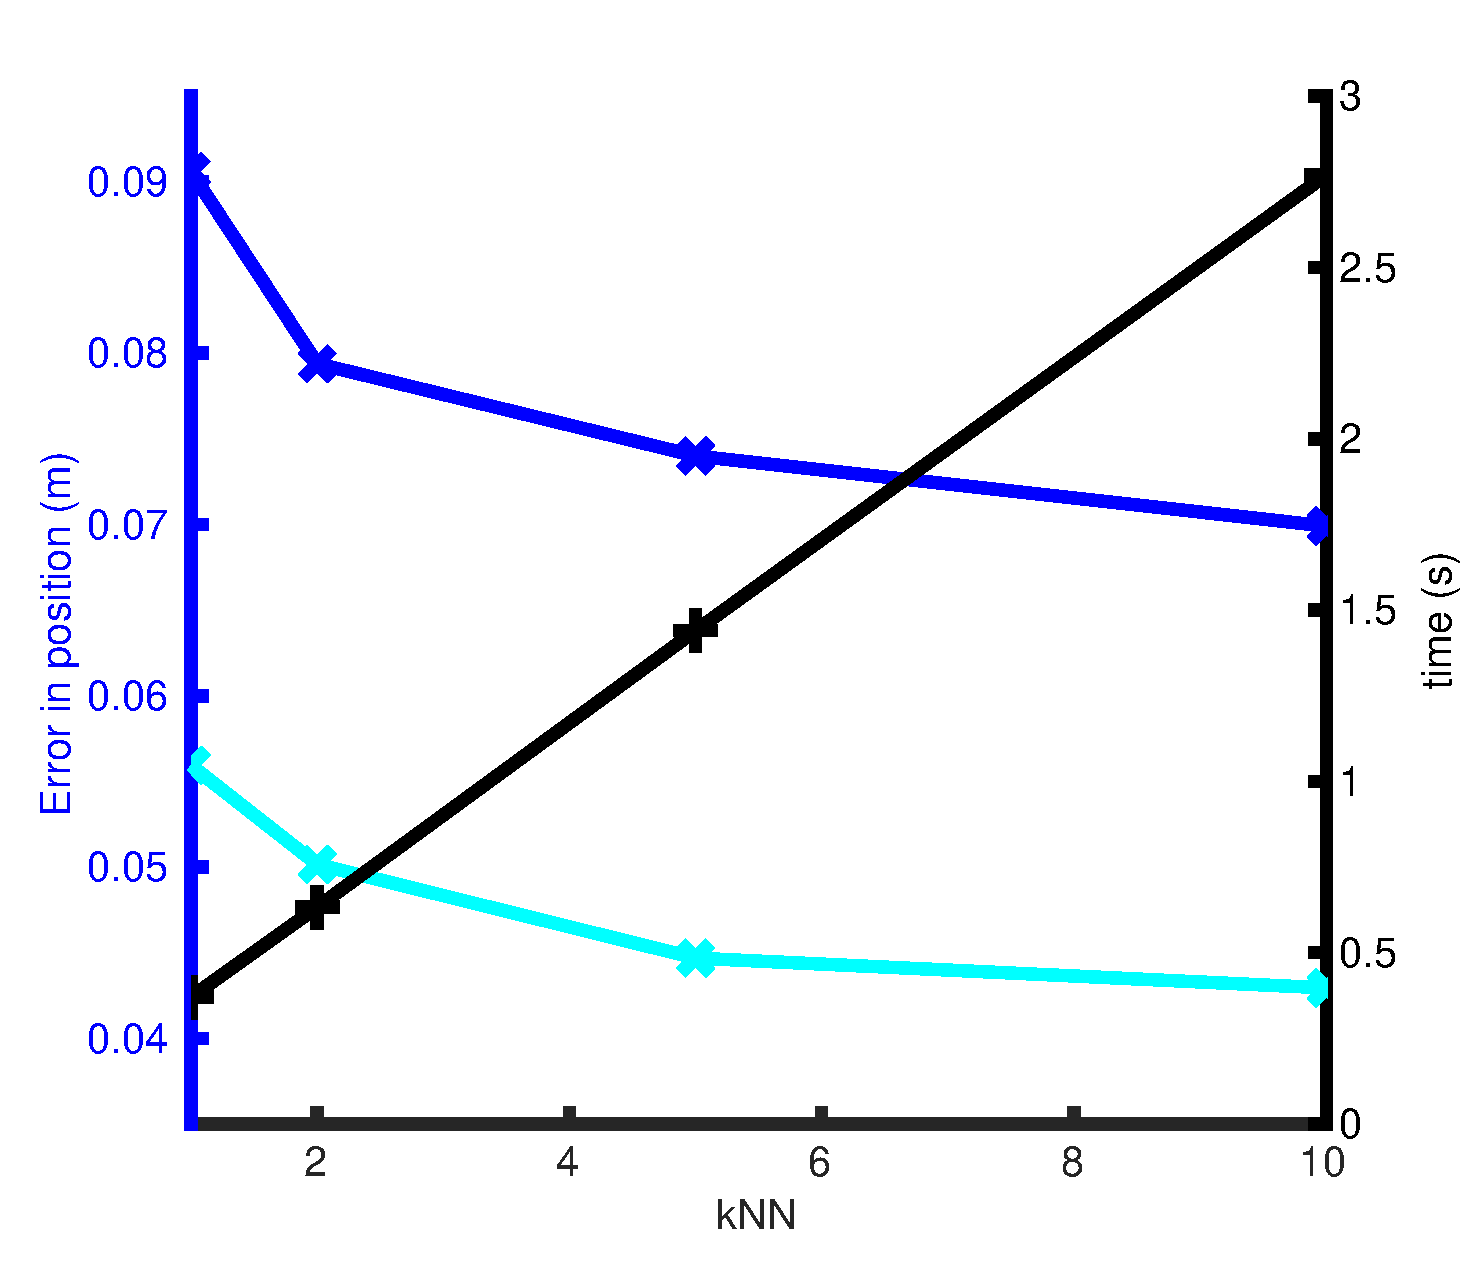
\includegraphics[width=\linewidth]{results/pos_err}
   		\end{minipage}\hfill
   		\begin{minipage}{0.5\linewidth}
   			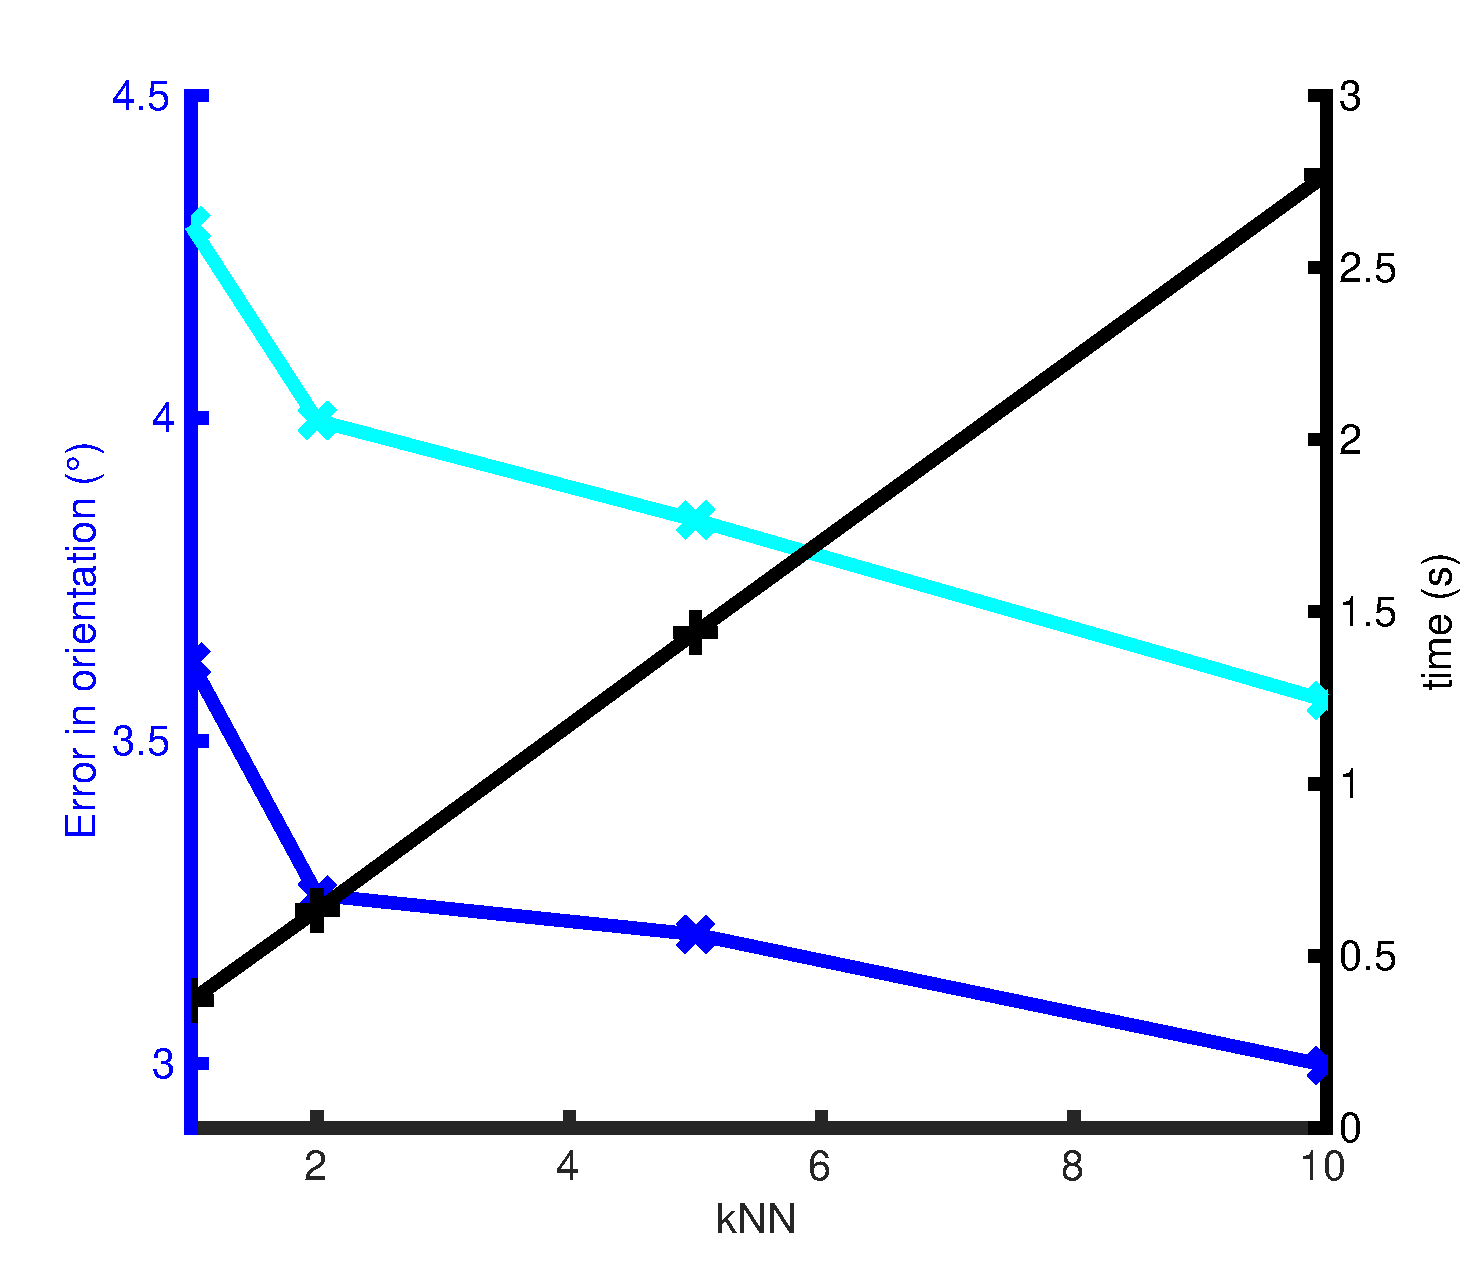
\includegraphics[width=\linewidth]{results/ori_err}
   		\end{minipage}
   		
   		\vspace{0.2cm}
   		
   		\begin{footnotesize}
   			\setlength{\tabcolsep}{2pt}
   			\begin{tabular}{c l c l c l}
   				\textcolor{red}{\Large{- -}} & NetVALD + RGB & \textcolor{blue}{\Large{- -}} & NetVALD + RGB(D)  & \textcolor{magenta}{\Large{- -}} & NetVALD + RGB(H)\\
   				\textcolor{red}{\Large{--}} & MAC + RGB & \textcolor{blue}{\Large{--}} & MAC + RGB(D) & \textcolor{magenta}{\Large{--}} & MAC + RGB(H)\\
   			\end{tabular}		
   		\end{footnotesize}
   		
   	\end{minipage}\hfill
   	\begin{minipage}{0.35\linewidth}
   		\caption[]{\label{fig:ratio_t_knn} .}
   	\end{minipage}	
	
	
	
\end{figure}
We report in table~\ref{tab:methods_comparison} initial result on the 7 scenes indoor dataset, using only the top-1 retrieved candidate for pose estimation for time saving. 

\paragraph{Initial localization.} We observe a comparable behavior than the one observed previously (section~\ref{sec:experiments}): NetVLAD pooling layer is more efficient than \ac{mac} for initial localization. In the following experiments, we only use the NetVLAD layer for global image descriptor. 

\paragraph{Deep descriptor.}
As we can see on the $x^{th}$ and $y^{th}$ columns of table~\ref{tab:methods_comparison}, using deep descriptors as well as 3D-point coordinates helps to form good matches, as expected in section~\ref{subsec:pc_alignment}.

\paragraph{\ac{iclp} vs \ac{pnlp}.} Our \ac{pnlp} pose refinement clearly outperform the \ac{iclp} approaches. This can be explained by the fact that wrong estimations in the depth map values are penalizing twice the \ac{iclp} approach and only once the \ac{pnlp} refinement. Thus, in the following, we use only the \ac{pnlp} pose estimation for refinement.

\paragraph{Number of retrieved candidates.} We use two scenes of the 7 scenes dataset to evaluate the impact of the number $K$ of retrieved candidates on the final localization. Figure~\ref{fig:ratio_t_knn} plot improvement for 4 values of $K$, from 1 to 10. We found that $K=5$ is a good trade-off between pose precision and time consumption. Localizing a query takes approximately one second using our non-optimized python code, including the image indexing step.